\section{Evaluation}\label{sec:evaluation}

In this section we evaluate our solution to the project mining problem, and show results for the example presented in Section~\ref{sec:background}.

\subsection{Experimental setup}

%
%This section should clarify the objective of the evaluation. What do we try to study with the evaluation (which quality characteristics)? This also relates to the question whether we let the result speak for itself or if we benchmark with competing approaches. here, you should also mention that the technique was implemented as a prototype.

We evaluate our technique by a visual perspective and by comparison to possible different approaches. To this end we implemented our technique as a prototype. We used JAVA as a programming language to code the logic of our technique. For the visualization part we made use of custom SWT widgets provided by the Nebula Project\footnote{https://www.eclipse.org/nebula/}. Our program can deal with logs from Subversion (SVN) \cite{pilato2008version} and Git\cite{torvalds2010git}, but it can be extended to other version control systems by providing an implementation of the preprocessing step discussed in Section~\ref{sec:subsec:discovery_technique}.
We ran the software in an Intel\textregistered Core \texttrademark~i5-4570 CPU @ 3.20 GHz x 4 machine with 15.6 GiB of RAM and Linux kernel 3.13.0-46-generic 64-bit version.

\subsection{Input data description}

We tested our prototype with real-world log data taken from the SHAPE project. Logs were exported from the SVN and Git repositories of different projects. They come from the railway domain and describe engineering processes. Documentation stored in the repositories consists of manually produced text files, diagrams, and files coming from proprietary tools that are typically used in the domain.

We will display results for the SVN log that describes the process oriented project for SHAPE. Data span over one year, going from January 2014 to January 2015. This time window covers the phases of project definition and planning, and a part of the project execution. In the first phase, feasibility of the project was studied and budget, schedule and resources were determined. Proposal submission marked the end of this phase. The second phase started with a kickoff meeting in October 2014 and is still ongoing.

The total number of participants who actively contributed to the work packages stored in the SVN repository was 8 people in the beginning, with new resources joining the project after the kickoff date. The total number of files and directories counts up to 156 objects and 226 overall commit events. The total number of extracted change events after preprocessing (i.e. atomic changes on all the files) was 453.

The last part of the log data contains the task \defineExample, introduced in Section~\ref{sec:problem}. For our showcase we assume that this task is contained in a work package named \emph{example}.

\subsection{Output data}

To monitor the project execution, we visualize the work progress that was done for each work package. Monitoring is performed by managers who want to have an overview on the project (which work packages are done, when and for how long, and where idleness or congestion occurs). Gantt charts offer a graphical representation for displaying schedules and jobs that were done on the various work packages \cite{wilson2003gantt} in a way that can easily be communicated to managers.

\begin{figure}
\centering
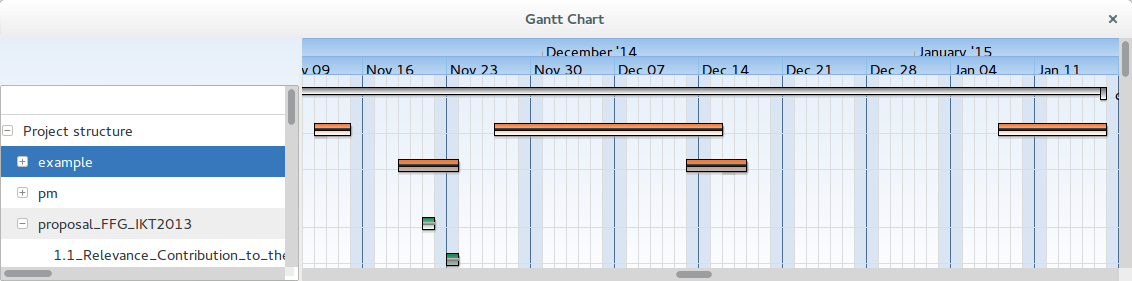
\includegraphics[width=\textwidth]{bpm2015/imgs/aggregation_and_not}
\caption{Data representation from our tool. Atomic events are drawn as dot with a minimal duration and different color per commit. }
\label{fig:example-screenshot}
\end{figure}

Figure~\ref{fig:example-screenshot} is a screenshot of how our tool presents the data. The tree structure on the left represents the \parent relation in the file tree. Events belonging to the same commit have the same color. On the top part of the chart we can see the result of merging events to activities with our aggregation method. Here we have merged the events of the example scenario on their highest abstraction level. The chart shows the three main activities and the idle times between them. %It is possible now to have an overview of the three main active periods in the work package.
On the other hand, in correspondence to expanded directories we show only their status before the aggregation. That is, every time a directory is fully expanded we apply a disaggregation into the corresponding activities. In this way, we can also show the finest granularity of work, i.e. the atomic events.

\subsection{Project Analysis}
Next, we apply our algorithm to the example case from Table~\ref{tab:example} and check how it helps to identify work packages. The data is aggregated according to our threshold of seven days. We can observe three groups of events being temporally close to each other according to our threshold. That is, we expect the event data to be grouped into three activities.

The second step of our algorithm takes care of adjusting the starting time of the activities. Furthermore, we vertically order the events and activities in the Gantt chart according to the directory structure to show the mapping from the objects on the Gantt chart to each work package in the tree structure. The last step, computing work package characteristics is done automatically when we collapse a node on of tree.

\begin{figure}
\centering
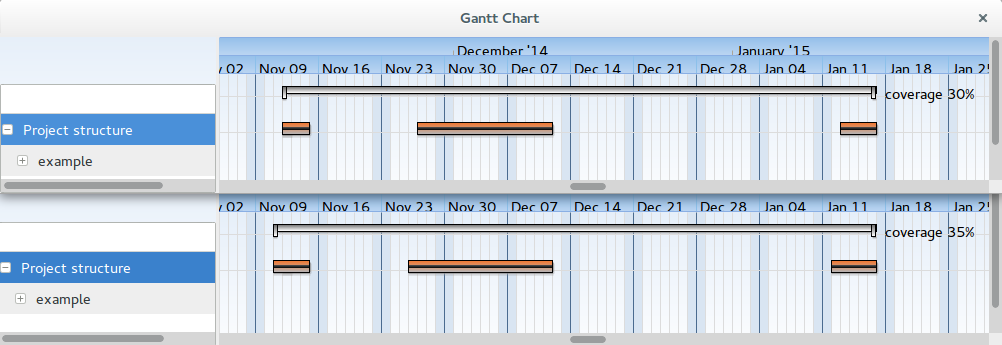
\includegraphics[width=\textwidth]{bpm2015/imgs/coverage_before_and_after}
\caption{Before and after the prepending the expected time before commit. Coverage factor increases when we adjust the starting times of the activities.}
\label{fig:example-collapsed}
\end{figure}

Figure~\ref{fig:example-collapsed} shows a comparison of the case when we do not implement the activity adjustment to the case which adjusts it. In the upper part, activity boundaries are based only on the first commit time that we see in the data. In the lower part, we observe that the start times were adjusted by approximately one day. The tool automatically adjusted the start time of the activities. As a consequence, the coverage factor increases because we expect that there was more work than what we observe by only considering the first commit time.

\subsection{Coverage tests on available open projects}

Finally, we apply our approach on different input data from open source projects. We are interested in exploring how the coverage factor varies in different existing projects. Hence, we take the work package $\workPackage$ as our controlled variable and set it to the highest level of aggregation. Then, we analyze each project of the data set and observe the dependent variable $\coverage(\workPackage)$.
Another variable of interest is the $\expectedActiveTime$ since it gives an idea of the average work speed (commit frequency) during active times.

\begin{table}
\caption{Coverage results for different open source projects}
\label{tab:experiments}
\centering
\begin{tabular}{rcccccc}
\hline\noalign{\smallskip}
\textbf{Log} ~&~ \textbf{Duration} ~&~ \textbf{Idle periods} ~&~ \textbf{Files} ~&~	 \textbf{Commits} ~&~	\textbf{$\expectedActiveTime$} ~&~ \textbf{$\coverage(\workPackage)$}\\
File name ~&~ Days ~&~ Number ~&~ Number ~&~ Number ~&~ Hours ~&~ \% \\
\hline \hline
\noalign{\medskip}
MiningCVS &	24 & 0 & 89  &	 63 & 9 & 100 \\
%\hline

Whitehall & 1279 & 6 & 6539  &	15566 & 2 & 95 \\
%\hline

Petitions &	834 & 17 & 1562  &	914 & 13 & 59 \\
%\hline

Study &	624 & 13 & 7501  &	736 & 11 & 58 \\
%\hline

The Guardian &	1667 & 59 & 12889  &	 621 & 30 & 44 \\
%\hline

Book &	414 & 15 & 154  & 592 & 5 & 32 \\
%\hline

Papers &	 1859 & 55 & 1791  &	 649 & 20 & 30 \\
%\hline

Requirements & 771 & 22 & 505  &	231 & 17 & 21 \\
%\hline

Yelp &	206 & 6 & 24  &	54 & 20 & 20 \\
%\hline

Adobe &	1076 & 13 & 356  &	237 & 24 & 15 \\
%\hline

\hline
\end{tabular}%\\ \hfill
\end{table}

%We test our tool on log data from open source projects that we find available on the web and data from SHAPE.
The data we used stems from the following projects. \emph{MiningVCS} is our tool. It consists of daily commits and was developed over 24 days.
\emph{Whitehall} is the code name for the Inside Government project, which aims to bring Government departments online in a consistent and user-friendly manner. \emph{Petitions} is a Drupal 7 code base used to build an application on "We The People", the platform to create and sign petitions of the White House.
\emph{Study} is an SVN log about Healthcare domain, taken from SHAPE.
\emph{The guardian} is the log data from the Git repository of the well-known British national daily newspaper.
\emph{Book} is the log data that describes the writing of the book Crypto 101 by Laurens Van Houtven, taken from Git.
\emph{Papers} is taken from SHAPE project for building a paper archive. %Reflects the history of collecting knowledge.
\emph{Requirements} log data is taken from the the Git repository of OpenETCS and belongs to the railway domain.
\emph{Yelp} is the main Github page of Yelp were they showcase all their projects.
\emph{Adobe} is the Adobe Github Homepage v2.0, which is a central hub for Adobe Open sources projects.

Table~\ref{tab:experiments} shows our experiments on the above-mentioned logs and the corresponding coverage factors. Projects that score a high coverage factor are characterized by continuous work. This can be further seen by looking at their average idle times $\avgIdleTime$. Let $n_c$ be the number of commits per work package. We compute the average idle time as follows.
\begin{equation}
\avgIdleTime = \frac{\durationOfWorkPackage  - n_c \cdot \expectedActiveTime }{n}
~,~ n>0
\end{equation}
where $n $ is the number of idle times in the work package. If $n=0$, then we trivially assign $\avgIdleTime = 0$, because there were no break periods over time.

Applying the formula to the above projects, we can observe how projects with a higher coverage factor have actually low values of $\avgIdleTime$. For instance, \emph{Whitehall} scores a $\avgIdleTime$ of 11 days, whereas \emph{Adobe} scores a $\avgIdleTime$ of 36 days.
This supports the usage of the coverage factor $\coverage$ as an indicator for work package time utilization. 